\section{Condenser Loop (\emph{Condenser Loop}) - Cooling Tower}\label{condenser-loop-condenser-loop---cooling-tower}

The Condenser Loop is constructed by using a \emph{PlantLoop} object. It uses a cooling tower (modeled by using a \emph{CoolingTower:SingleSpeed} object class) and a constant speed pump (modeled by using a \emph{Pump:ConstantSpeed)} to supply cooling water to the electric chiller (modeled by using a \emph{Chiller:Electric} object). Therefore, the supply side of the loop contains the Cooling Tower and the demand side contains the electric chiller. The loop is operated by using plant equipment operation schemes, and schedules. ~Refer to Figure~\ref{fig:simple-line-diagram-for-the-condenser-loop} for a simple diagram of the Condenser Loop.

\begin{figure}[hbtp] % fig 61
\centering
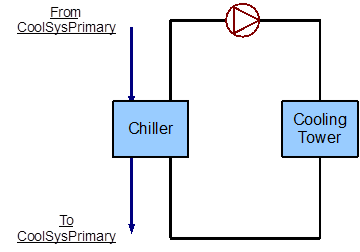
\includegraphics[width=0.9\textwidth, height=0.9\textheight, keepaspectratio=true]{media/image061.png}
\caption{Simple line diagram for the condenser loop \protect \label{fig:simple-line-diagram-for-the-condenser-loop}}
\end{figure}

\subsection{Flowcharts for the Condenser Loop Input Process}\label{flowcharts-for-the-condenser-loop-input-process}

This series of flowcharts serve as a guide for identifying and inputting the Condenser Loop and its components into the input file. The EnergyPlus line diagram for this loop is provided in Figure~\ref{fig:energyplus-line-diagram-for-the-condenser}. A simple flowchart for the separation of the half loops is provided in Figure~\ref{fig:simple-flow-chart-for-separation-on-half}.

\begin{figure}[hbtp] % fig 62
\centering
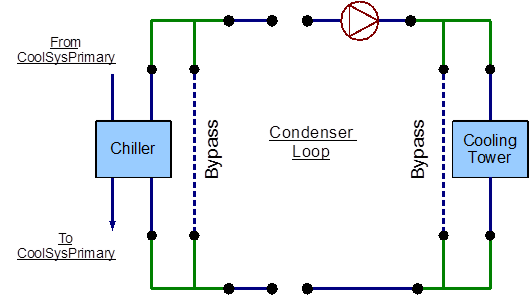
\includegraphics[width=0.9\textwidth, height=0.9\textheight, keepaspectratio=true]{media/image062.png}
\caption{EnergyPlus line diagram for the condenser loop \protect \label{fig:energyplus-line-diagram-for-the-condenser}}
\end{figure}

\begin{figure}[hbtp] % fig 63
\centering
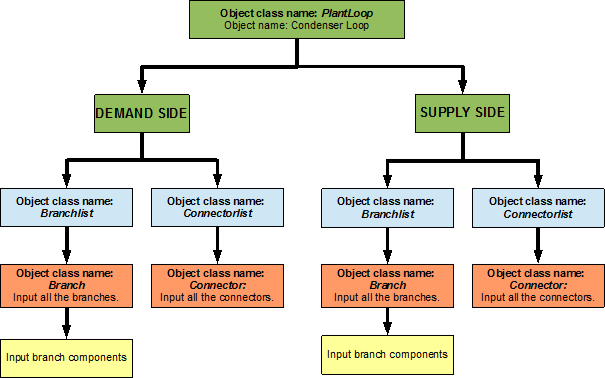
\includegraphics[width=0.9\textwidth, height=0.9\textheight, keepaspectratio=true]{media/image063.png}
\caption{Simple flow chart for separation on half loops in the condenser loop \protect \label{fig:simple-flow-chart-for-separation-on-half}}
\end{figure}

\subsubsection{Condenser Loop Supply Side Construction}\label{condenser-loop-supply-side-construction}

The main components on the supply side half loop for the Condenser Loop are the Cooling Tower that supplies the cooling water and the constant speed pump that circulates the cooling water through the loop. This half loop supplies cooling water to the electric chiller on the demand side half loop. The supply side half loop contains four components, four branches, eight nodes, and one splitter-mixer pair. The EnergyPlus line diagram for the Condenser loop supply side is provided in Figure~\ref{fig:energyplus-line-diagram-for-the-supply-side-001}. The flowchart for supply side branches and components is provided in Figure~\ref{fig:flowchart-for-condenser-loop-supply-side-branches-and}. The flowchart for supply side connectors is provided in Figure~\ref{fig:flowchart-for-condenser-loop-supply-side-connectors}.

\begin{figure}[hbtp] % fig 64
\centering
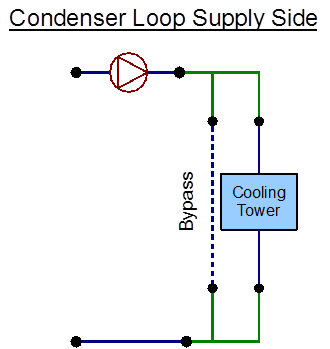
\includegraphics[width=0.9\textwidth, height=0.9\textheight, keepaspectratio=true]{media/image064.png}
\caption{EnergyPlus line diagram for the supply side of the condenser loop \protect \label{fig:energyplus-line-diagram-for-the-supply-side-001}}
\end{figure}

\begin{figure}[hbtp] % fig 65
\centering
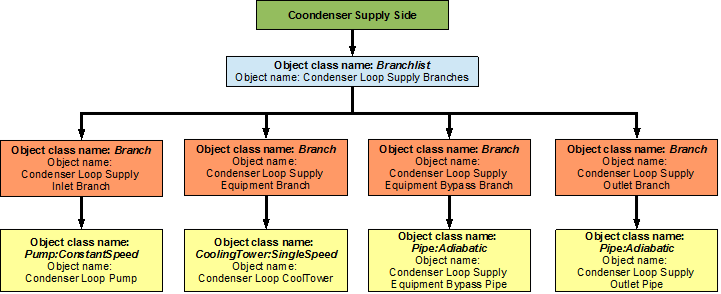
\includegraphics[width=0.9\textwidth, height=0.9\textheight, keepaspectratio=true]{media/image065.png}
\caption{Flowchart for condenser loop supply side branches and components \protect \label{fig:flowchart-for-condenser-loop-supply-side-branches-and}}
\end{figure}

\begin{figure}[hbtp] % fig 66
\centering
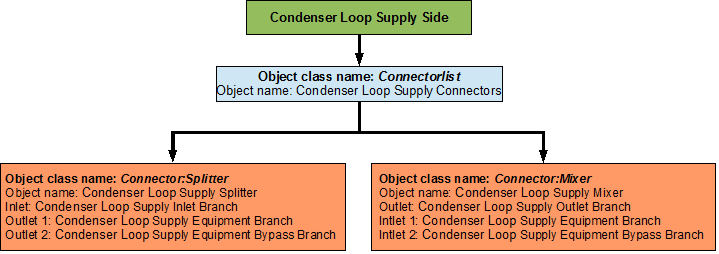
\includegraphics[width=0.9\textwidth, height=0.9\textheight, keepaspectratio=true]{media/image066.png}
\caption{Flowchart for condenser loop supply side connectors \protect \label{fig:flowchart-for-condenser-loop-supply-side-connectors}}
\end{figure}

\subsubsection{Condenser Loop Demand Side Construction}\label{condenser-loop-demand-side-construction}

The main component on the demand side half loop is the Chiller that uses the cooling water supplied by the cooling tower. The chiller in turn is used to supply chilled water in the Primary Cooling loop. ~This side of the loop also has eight nodes, four components, four branches and one splitter-mixer pair. An EnergyPlus schematic for the demand side is provided in Figure~\ref{fig:energyplus-line-diagram-for-the-demand-side-001}. The flowchart for demand side branch definition is provided in Figure~\ref{fig:flowchart-for-condenser-loop-demand-side-branches-and}. The flowchart for the demand side connectors is provided in Figure~\ref{fig:flowchart-for-condenser-loop-demand-side-connectors}.

\begin{figure}[hbtp] % fig 67
\centering
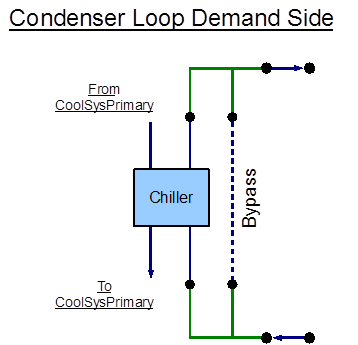
\includegraphics[width=0.9\textwidth, height=0.9\textheight, keepaspectratio=true]{media/image067.png}
\caption{EnergyPlus line diagram for the demand side of the condenser loop \protect \label{fig:energyplus-line-diagram-for-the-demand-side-001}}
\end{figure}

\begin{figure}[hbtp] % fig 68
\centering
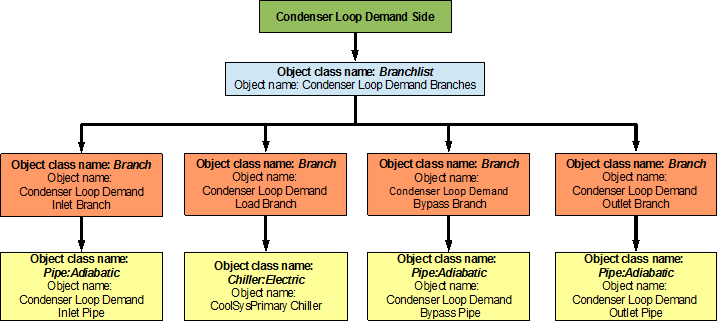
\includegraphics[width=0.9\textwidth, height=0.9\textheight, keepaspectratio=true]{media/image068.png}
\caption{Flowchart for condenser loop demand side branches and components \protect \label{fig:flowchart-for-condenser-loop-demand-side-branches-and}}
\end{figure}

\begin{figure}[hbtp] % fig 69
\centering
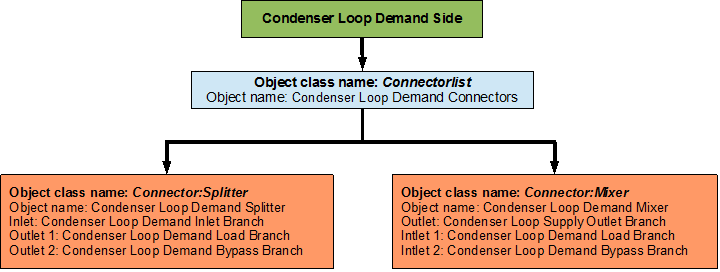
\includegraphics[width=0.9\textwidth, height=0.9\textheight, keepaspectratio=true]{media/image069.png}
\caption{Flowchart for condenser loop demand side connectors \protect \label{fig:flowchart-for-condenser-loop-demand-side-connectors}}
\end{figure}

\subsection{Flowcharts for Condenser Loop Controls}\label{flowcharts-for-condenser-loop-controls}

The Condenser Loop is operated by using set-points, plant equipment operation schemes and schedules.

\subsubsection{Condenser Loop Schedules}\label{condenser-loop-schedules}

The flowchart for condenser loop schedule definition is provided in Figure~\ref{fig:flowchart-for-condenser-loop-schedules}. The Condenser loop uses one schedule to operate properly. \emph{PlantOnSchedule} is a compact schedule that keeps the Cooling Tower On at all times of the day, this compact schedule uses a discrete \emph{ScheduleTypeLimit} (\emph{On/Off)} which defines that the value of On is 1 and that of Off is 0.

\begin{figure}[hbtp] % fig 70
\centering
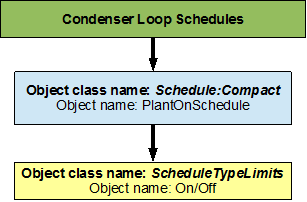
\includegraphics[width=0.9\textwidth, height=0.9\textheight, keepaspectratio=true]{media/image070.png}
\caption{Flowchart for condenser loop schedules \protect \label{fig:flowchart-for-condenser-loop-schedules}}
\end{figure}

\subsubsection{Condenser Loop Plant Equipment Operation Schemes}\label{condenser-loop-plant-equipment-operation-schemes}

The \emph{PlantEquipmentOperationschemes} object uses the \emph{PlantOnSchedule} and the \emph{Condenser Loop Operation Scheme} objects to set the range of demand loads for which the cooling tower is operated during the simulation period. A flowchart detailing the Condenser Loop plant equipment operation schemes is provided in Figure~\ref{fig:flowchart-for-condenser-loop-plant-equipment-operation}.

\begin{figure}[hbtp] % fig 71
\centering
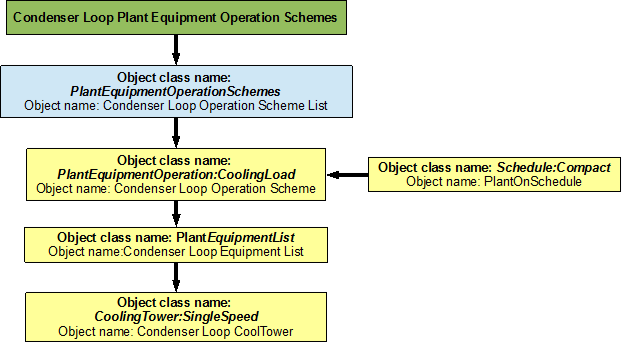
\includegraphics[width=0.9\textwidth, height=0.9\textheight, keepaspectratio=true]{media/image071.png}
\caption{Flowchart for condenser loop plant equipment operation schemes \protect \label{fig:flowchart-for-condenser-loop-plant-equipment-operation}}
\end{figure}

\subsubsection{Condenser Loop Setpoints}\label{condenser-loop-setpoints}

The \emph{MyCondenserControl} setpointmanager places a temperature setpoint at the \emph{Condenser Supply Outlet Node.} The temperature at this point is controlled with respect to the outdoor air wet bulb temperature at that point in the simulation. The outdoor air wet bulb temperature is obtained from the weather data at the location of the simulation. The minimum setpoint temperature is 5 degrees Celsius and the maximum setpoint temperature is 80 degrees Celsius. A flowchart for Secondary Cooling loop setpoints is provided in Figure~\ref{fig:flowchart-for-condenser-loop-setpoints}.

\begin{figure}[hbtp] % fig 72
\centering
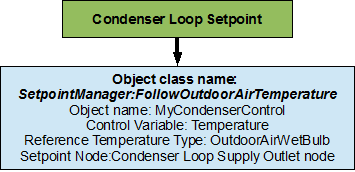
\includegraphics[width=0.9\textwidth, height=0.9\textheight, keepaspectratio=true]{media/image072.png}
\caption{Flowchart for condenser loop setpoints \protect \label{fig:flowchart-for-condenser-loop-setpoints}}
\end{figure}

\subsubsection{Condenser Loop Sizing}\label{condenser-loop-sizing}

The Condenser loop is sized such a way that the design loop exit temperature is 29.4 degrees Celsius, and the loop design temperature difference is 5.6 degrees Celsius. A flowchart for the chilled water loop sizing is provided in Figure~\ref{fig:flowchart-for-condenser-loop-sizing}.

\begin{figure}[hbtp] % fig 73
\centering
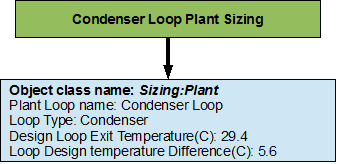
\includegraphics[width=0.9\textwidth, height=0.9\textheight, keepaspectratio=true]{media/image073.png}
\caption{Flowchart for condenser loop sizing \protect \label{fig:flowchart-for-condenser-loop-sizing}}
\end{figure}
